\paragraph{}
A data set (or dataset) is a collection of data, Most commonly a data set corresponds to the contents of a single database table, where each column of the table represents a particular variable(feature), when working in machine learning we need datasets for training our models, huge datasets are preferred sometimes specially for deep learning.\newline
\subsubsection{Brief of used Datesets.}
\textbf{FER13}
\begin{figure}
	\centering
	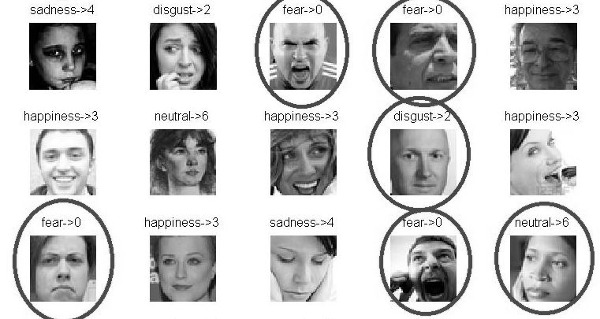
\includegraphics[width=.7\textwidth]{images/fer2013.jpg}
	\caption{samples from fer13 dataset.}
\end{figure} 
\paragraph{}
FER2013 is a large, publicly available Facial Expression Detection dataset consisting of 35,887 face crops, The dataset is challenging as the depicted faces vary significantly in terms of person age, face pose, and other factors, reflecting realistic conditions, 
The dataset is split into training, validation, and test sets with 28,709, 3,589, and 3,589 samples respectively.(see Figure \ref{fig:fer13})\newline
fer13 contains seven categories (0=Angry, 1=Disgust, 2=Fear, 3=Happy, 4=Sad, 5=Surprise, 6=Neutral), Basic expression labels are provided for all samples, All images are grayscale and have a resolution of 48 by 48 pixels, The human accuracy on this dataset is around 65.5\%. 
 
\begin{figure}
	\centering
	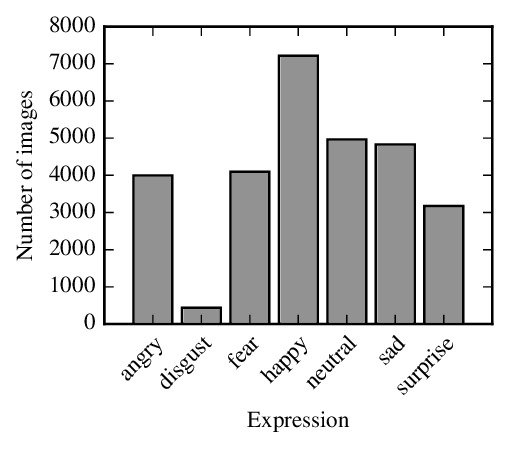
\includegraphics[width=.5\textwidth]{images/fer_dis.png}
	\caption{Fer13 imbalanced distribution}
	\label{fig:fer13}
\end{figure} 
\paragraph{}
from Figure \ref{fig:fer13} which describe the the distribution of data in the dataset and the information provided in the dataset description we notice that :
\begin{enumerate}
	\item the dataset contain a lot of images that is not faces or can't be detected with the available techniques in openCV.
	\item there is unbalanced distribution of data ("disgust" emotion has only 500 images while happy has around 7000 images)   
\end{enumerate}

 This makes the classification harder because the model have to generalize well and be robust to incorrect data, The best accuracy results obtained on this dataset is 75.2\% according to this paper:\cite{state_of_art}[Facial Expression Recognition using Convolutional Neural Networks: State of the Art, Pramerdorfer \& al. 2016] using CNN .

\subsubsection{CK+}
\paragraph{}
Extended cohen kandle dataset is a small dataset ,publicly available Facial Expression Detection dataset Participants are 18 to 50 years of age, 69\% female, 81\% Euro-American 
13\% Afro-Americn and 6\% other groups .
\paragraph{}
Image sequances for frontal views and 30-degree views were digitalized into either 640*940 or 640*480 pixel arrays with 8-bit gray scale or 124 color value.contains eight categories neutral, sadness, surprise, happiness, fear, anger, contempt and disgust.

\subsubsection{Radrubd}
\paragraph{}
an academic dataset contain 1308 image for 8 emotions each emotion have 200 image , each person in this dataset asked to make 8 emotion then record his emotion from three directions with good resolution .
